\documentclass[10pt]{beamer}
%\usetheme{Amsterdam}
\usetheme{Darmstadt}
%\usecolortheme{beaver}

%Include all packages
%\ProvidesPackage{./tex/mySlideShowStyle}
%Packages pour les langues
\usepackage[utf8]{inputenc}
\usepackage[frenchb]{babel}
\usepackage[T1]{fontenc}
\usepackage{float}
\usepackage{lmodern}
\usepackage{multimedia}

%Package pour la mise en forme
\usepackage{parallel}
\usepackage{setspace}
\usepackage{wrapfig}
\usepackage{color, colortbl}

%Packages pour les liens dynamiques
\usepackage{hyperref}
\usepackage{multicol}
%\usepackage{underscore}

%Packages pour les formules de Maths
\usepackage{amsmath}
\usepackage{amsfonts}
\usepackage{amssymb}
\usepackage{mathrsfs}
\usepackage{mathtools}
\usepackage{mathabx}
\usepackage{pseudocode}
\usepackage{fancybox}

%Packages des images
\usepackage{graphicx}
%\usepackage{subfigure}
\usepackage{subfig}
\usepackage{wrapfig}
\usepackage{caption}
%\usepackage{subcaption}

%Packages pour les string
\usepackage{xstring}

%Packages pour les listes
%\usepackage{enumitem}
\usepackage{moreverb}



%%%%%%%%%%%%%%%%%
\author{Nuno Guedelha}
\title{Implémentation et application d'un algorithme de Dynamique Hybride}
%\setbeamercovered{transparent} 
\setbeamertemplate{navigation symbols}{} 
%\logo{} 
\institute{LAAS-CNRS}
\date{} 
%\subject{} 

\setbeamertemplate{footline}{
\leavevmode%
\hbox{\hspace*{-0.06cm}
\begin{beamercolorbox}[wd=.2\paperwidth,ht=2.25ex,dp=1ex,center]{author in head/foot}%
	\usebeamerfont{author in head/foot}\insertshortauthor%~~(\insertshortinstitute)
\end{beamercolorbox}%
\begin{beamercolorbox}[wd=.55\paperwidth,ht=2.25ex,dp=1ex,center]{section in head/foot}%
	\usebeamerfont{section in head/foot}\insertshorttitle
\end{beamercolorbox}%
\begin{beamercolorbox}[wd=.25\paperwidth,ht=2.25ex,dp=1ex,right]{section in head/foot}%
	\usebeamerfont{section in head/foot}\insertshortdate{}\hspace*{2em}
	\insertframenumber{} / \inserttotalframenumber\hspace*{2ex}
\end{beamercolorbox}}%
\vskip0pt%
}

\begin{document}


%==========================================================
%=============== variable fichier de figures ==============================

\newcommand{\myFiguresFile}{}
\newcommand{\setmyFiguresFile}[1]{\renewcommand{\myFiguresFile}{#1}}

%=============== include 1 figure =========================================

\ifx \incFig \undefined
\def \incFig [#1]#2{\includegraphics[width=#2, page=#1]{figs/\myFiguresFile}}
\fi

%=============== Display 1 figure =========================================

\ifx \dispFig \undefined
\def \dispFig [#1]#2#3#4#5%
{
\begin{figure}[#1]
  \begin{center}
  \includegraphics[width=#3, page=#2]{figs/\myFiguresFile}
  \IfStrEq{#4}{}{}{%
    \caption{#4}  % legende
    \label{#5}    % pour citer le numéro de figure
  }
  \end{center}
\end{figure}
}
\fi

%=============== 2 sous-figures alignées horizontalement =================

\ifx \dispTwoFig \undefined
\def \dispTwoFig [#1]#2#3#4#5#6#7%
{
\begin{figure}[#1]
\begin{center}
  \subfloat[#3 \label{#7.a}]{\includegraphics[width=7cm, page=#2]{figs/\myFiguresFile}}\hspace{1cm}
  \subfloat[#5 \label{#7.b}]{\includegraphics[width=7cm, page=#4]{figs/\myFiguresFile}}\hspace{1cm}
  \caption{#6}  % legende \\
  \label{#7} % pour citer le numéro de figure
\end{center}
\end{figure}
}
\fi

%=============== 3 sous-figures alignées horizontalement =================

\ifx \dispThreeFig \undefined
\def \dispThreeFig [#1]#2#3#4#5#6#7#8#9%
{
\begin{figure}[#1]
\begin{center}
  \subfloat[#3 \label{#9.a}]{\includegraphics[width=5cm, page=#2]{figs/\myFiguresFile}}\hspace{1cm}
  \subfloat[#5 \label{#9.b}]{\includegraphics[width=5cm, page=#4]{figs/\myFiguresFile}}\hspace{1cm}
  \subfloat[#7 \label{#9.c}]{\includegraphics[width=5cm, page=#6]{figs/\myFiguresFile}}\\
  \caption{#8}  % legende
  \label{#9}    % pour citer le numéro de figure
\end{center}
\end{figure}
}
\fi

%=============== 2 ou 3 colonnes alignée horizontalement ==================

\ifx \minipages \undefined
\def \minipages [#1]#2#3#4#5#6#7#8%
{
\begin{minipage}[#2]{#3\textwidth}
  #6
\end{minipage}
\begin{minipage}[#2]{#4\textwidth} \hfill
  #7
\end{minipage}
\IfStrEq{#1}{3}%
{
\begin{minipage}[#2]{#5\textwidth} \hfill
  #8
\end{minipage}
}
}
\fi

%=============== exemples ==================================================

%\begin{minipage}{.3\textwidth} \hfill
%  \begin{align*}
%  D_{O} = \lbrace &\textbf{d}_{Ox}, \textbf{d}_{Oy}, \textbf{d}_{Oy}, \\
%  &\textbf{d}_{x}, \textbf{d}_{y}, \textbf{d}_{z} \rbrace \subset M^{6}
%  \end{align*}
%\end{minipage}
%\begin{minipage}{.4\textwidth} \hfill
%  \begin{tabbing}
%  \= $\textbf{d}_{Ox}$ \= vecteur unitaire de rotation autour de $O_{x}$\\
%  \> $\textbf{d}_{Oy}$ \> vecteur unitaire de rotation autour de $O_{y}$\\
%  \> $\textbf{d}_{Oz}$ \> vecteur unitaire de rotation autour de $O_{z}$\\
%  \> $\textbf{d}_{x}$  \> vecteur unitaire de translation le long de $O_{x}$\\
%  \> $\textbf{d}_{y}$  \> vecteur unitaire de translation le long de $O_{y}$\\
%  \> $\textbf{d}_{z}$  \> vecteur unitaire de translation le long de $O_{z}$\\
%  \end{tabbing}
%\end{minipage}

%=============== autres macro textuelles ===================================

\newcommand{\cad}[0]{\textnormal{c'est à dire }}

\newcommand{\fd}[0]{\emph{fd}}

\newcommand{\mfd}[0]{\mathit{fd}}

\newcommand{\valTextwidth}[0]{\thetextwidth}

\newcommand{\valTextwidthUnit}[1]{\printinunitsof{#1}\prntlen{\textwidth}}

\newcommand{\valInUnit}[2]{\printinunitsof{#1}\prntlen{#2}}

%affichage des largeurs de zone texte
%\usepackage{layouts}
%\printinunitsof{cm}\prntlen{\textwidth}

\newcommand{\newglossdef}[3]
{\newglossaryentry{#1}%
{%
  name={#2},%
  description={#3}%
}}

%	\begin{frame}[allowframebreaks]{Title}
%	...
%	\framebreak
%	...
%	\end{frame}


%==========================================================

\begin{frame}
\titlepage
\end{frame}
%==========================================================

\begin{frame}{Plan}
\tableofcontents[part=01]
\tableofcontents[part=02]
\end{frame}
%==========================================================

\part{}

\section{Introduction}

\begin{frame}
  \frametitle{Contexte du stage}
  \framesubtitle{}
  \begin{block}{Projet professionnel}
  \begin{itemize}
    \item première expérience dans l'embarqué et le temps réel
    \item nouveau cap: la robotique mobile et le Master 2 IRR
    \item Objectif: chercheur en Robotique (entreprise ou laboratoire)
  \end{itemize}
  \end{block}
  \begin{block}{Le LAAS et Gepetto}
  \begin{itemize}
    \item Gepetto: expertise en analyse, génération de mouvements  
    \item Approche fondamentale, modélisation dynamique, contrôle, planification de mouvements
    \item {Intégration dans des packages open source \\
          $\hookrightarrow$ metapod: librairie de modélisation dynamique}
    \note{}
  \end{itemize}
  \end{block}
\end{frame}

\begin{frame}
  \frametitle{Objectifs}
  
  \begin{block}{Implémentation d'un algorithme de dynamique hybride dans metapod:}
	\begin{itemize}
		\item formalisme de Newton-Euler, Algèbre Spatiale
\note{vs formalisme Lagrange: effort généralisé sur chaque articulation en termes d'NRJ}
		\item algorithmes et optimisation de Roy Featherstone
\note{Roy Featherstone: (“Rigid Body Dynamics Algorithm",2008) Chercheur spécialisé en modélisation dynamique de robots. Ph.D. à Edinburgh -> univ Australian National -> Professeur invité à l'IIT}
		\item C++ template méta-programmation
		\item combiner à Eigen \note{librairie templatée}
		\item benchmarking
  \end{itemize}
  \end{block}
	
	\bigskip
  Réflexion sur l'application de la Dynamique Hybride:
  	\begin{itemize}
		\item modélisation d'articulations flexibles ("compliant")
		\item commande de robot ayant une base flottante
  \end{itemize}
	
\end{frame}
%==========================================================

\section{Modélisation Dynamique}

\begin{frame}[allowframebreaks]
  \frametitle{Cas d'utilisation}
  
  Indispensable $\begin{cases}  \text{compenser l'inertie des membres} \\ 
                                \text{garantir l'appui au sol} \end{cases}$ \note{robot sans base fixe} \\
  
  \bigskip
  Composantes de l'équation de mouvement:
  	\begin{description}
	  \item[$model$ :] le modèle dynamique du système à multi-corps rigides
	  \item[$\bsy{q, \dot{q}, \ddot{q}}$ :] vecteurs de position, vitesse, accélération des articulations du système
	  \item[$\bsy{\tau}$ :] forces/couples moteurs (internes) appliqués aux articulations
	  \item[$\bsy{f^{ext}}$ :] forces de contrainte extérieures (force de gravitation, coriolis, forces de contact, ...)
	\end{description}
	
	\framebreak

  \setmyFiguresFile{hrp2Control}
	
	3 types de problèmes dynamiques et applications:
	\begin{figure}[T]
	\begin{columns}[T]
	  \begin{column}{.48\textwidth}
		  \begin{itemize}
		  	\item dynamique directe \\
		  	      $\rightarrow$ \href{run:/home/nuno/Documents/Stage/Documents/Videos/14-ichr-metapod-v6-submitted.mp4}	{\textcolor{blue}{simulation}}:
		  	      \note{trouver les accélérations induites par les forces appliquées aux articulations}
						\begin{equation}
						\ddot{q} = \mathrm{FD}(model,\bsy{q,\dot{q},\tau})
						\end{equation}
		  \item 	dynamique inverse \\
		        $\rightarrow$ contrôle du \emph{CoM} (compense l'inertie des bras):
		        \note{trouver les forces à appliquer aux accélérations pour produire les articulations voulues. Estimation du centre de pression $\longrightarrow$ injecté dans le PC (preview control) $\longrightarrow$ générer trajectoire CoM}
						\begin{equation}
						\bsy{\tau} = \mathrm{ID}(model,\bsy{q,\dot{q},\ddot{q}})
						\end{equation}
			\end{itemize}
		\end{column}
		\begin{column}{.48\textwidth}
		  \begin{center}
		  \href{run:/home/nuno/Documents/Stage/Documents/Videos/14-ichr-metapod-v6-submitted.mp4}{\includegraphics[width=.5\textwidth, page=1]{figs/\myFiguresFile}} \\
		  \bigskip
			\href{run:/home/nuno/Documents/Stage/Documents/Videos/14-ichr-metapod-v6-submitted.mp4}{\includegraphics[width=.5\textwidth, page=1]{figs/\myFiguresFile}}
			\hfill
			\end{center}
		\end{column}
	\end{columns}
	\end{figure}
	
	\hyperlink{app_filDyn}{\beamergotobutton{(i)}}
  
	\framebreak
	
	\begin{block}{}
	\begin{spacing}{1.2}
	\begin{itemize}
	\item Dynamique hybride (CHDA): généralisation de l'ID et de la FD.\\
	      $\rightarrow$ Simulation + fidèle (flexibilité) \\
        $\rightarrow$ Simulation simplifiée (articulations "parfaites") \\
        $\rightarrow$ Améliorer contrôle de robots à base flottante \\
                      $\hookrightarrow$ $\tau_0$ connu = 0 $\rightarrow$ calcul de $\ddot{q}_0$! \\
                                        (estimation du CoM affinée)
\note{pour chaque articulation, on connaît soit le couple (art. $fd$) soit l'accélération (art. $id$). L'algo calcule toutes les inconnues ($fd$ $\longrightarrow$ FD, $id$ $\longrightarrow$ ID)}
  \end{itemize}
  \end{spacing}
  \end{block}
	
	\begin{equation}
	\bsy{\begin{bmatrix} \ddot{q}_1 \\ \ddot{q}_2	\end{bmatrix}}, \bsy{\begin{bmatrix} \tau_1 \\ \tau_2	\end{bmatrix}} = \mathrm{CHDA}(model,\bsy{q,\dot{q},\begin{bmatrix} 0 \\ \ddot{q}_2	\end{bmatrix},\begin{bmatrix} \tau_1 \\ 0	\end{bmatrix}})
	\end{equation}
	
\end{frame}

%==========================================================

\section{Contraintes en performances}

\begin{frame}
  \frametitle{Contraintes et méta programmation}

	\begin{block}{Cahier des charges du RNEA}
	Vitesse:
	\begin{itemize}
	\item fenêtre de filtrage dynamique 1.6s $\longrightarrow$ 32 RNEA /s
	\item < v > ~ $4\mu s$ sur i7-4700HQ, ~ $15\mu s$ sur HRP2 Core2(TM) Duo E7500
	\end{itemize}
	
	précision numérique: 0.1%
	\end{block}
	
\end{frame}

\begin{frame}
  \frametitle{Algèbre Spatiale et méta programmation}
  
  \begin{itemize}
  \item basée sur les torseurs (avec différence de notation), réduit la compléxité de la modélisation dynamique, comb. translation/rotation \\
        (composition simplifiée des vitesses et accélérations)
  \item Algos CRBA et RNEA exploitent la récursivité (\emph{pattern} Visiteur), la "sparsité" / abscesnce de couplage entre branches cinématiques
  \item méta prog. => propriétés d'un langage symbolique (calculs inutiles non exécutés)
  \item méta fonctions génèrent des traitements/calculs numériques à la compilation \\
        (conditions méta fonction: params->types ou int statiques et constants)
  \end{itemize}
  
\end{frame}

\begin{frame}
  \frametitle{Génération automatique d'algorithmes optimisés et spécialisés}
  
	\begin{figure}[H]
	\begin{center}
	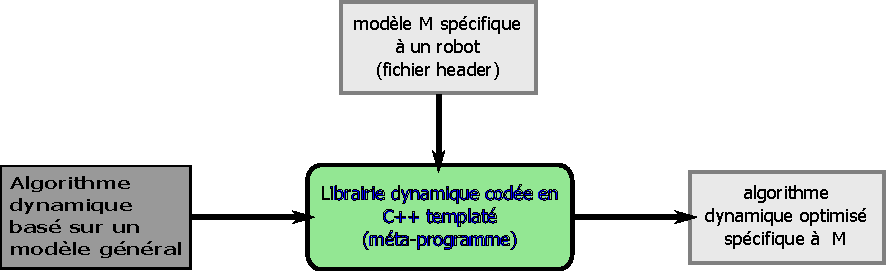
\includegraphics[width=\textwidth]{figs/principeAlgoGenerique.pdf}
	\label{fig_generationAlgoAutomatique}
	\end{center}
	\end{figure}
  
\note{	\emph{metapo} fournit algos basés sur modèle dynamique général \\
      	prend un modèle $M$ spécifique (header) \\
     	génère du code optimisé spécifique au modèle $M$}
	
	\bigskip
	%lien vers schéma fonctionnel interne de metapod
	\href{run:/home/nuno/Documents/Stage/Soutenance/figs/archiMetapod.pdf}
	{($\downarrow$ \textcolor{blue}{schéma fonctionnel interne de metapod})}

\end{frame}

%==========================================================

\section{Algèbre Spatiale et construction d'un arbre cinématique}

\subsection{Formalisme de l'Algèbre Spatiale}
\setmyFiguresFile{figures}

\begin{frame}
  \frametitle{}
  
  \begin{block}{Formalisme basé sur la mécanique des torseurs}
  \begin{spacing}{1}
  \note{Notations simplifiées et spécifiques à Featherstone}
  \begin{itemize}
	  \item vitesse spatiale $\widehat{v} \iff$ torseurs de mouvement
	        \note{%
	        $\widehat{v}_O = $ vitesse du flux de points du corps à travers $O$ \\
	        vecteur = $\omega$, moment = $v_O$ \\
	        ensemble de vecteurs liés => champ antisymétrique}
	  \item force spatiale $\widehat{f} \iff$ torseur de force
	  \item composition des vitesses, forces $\longrightarrow$ \textbf{additive}:
	  \begin{description}
	    \item[vitesse:] translation + rotation d'un seul corps \\
	                    vitesse relative enfant / parent
	    \item[force:] couple + force linéaire \\
	                  force à travers une articulation
	  \end{description}
  \end{itemize}
  \end{spacing}
  \end{block}
  
  \begin{columns}[onlytextwidth]
    \begin{column}{.5\textwidth}\footnotesize
		  rotation $\omega \rightarrow \widehat{v}_O = \bsy{\begin{bmatrix} \omega \\ v_O = OP \times \omega \end{bmatrix}} \quad$ \\
		  translation $v_p \rightarrow \widehat{v}_O = \bsy{\begin{bmatrix} 0 \\ v_O = v_P \end{bmatrix}}$
    \end{column}
    \begin{column}{.5\textwidth}
      \vspace{-0.5cm} \dispFig[H]{1}{\textwidth}{}{vitesseSpatiale}
    \end{column}
  \end{columns}
  
\end{frame}

\begin{frame}
  \frametitle{}
  
  \note{
  force f en p  => fo=[n0=op x f; f] \\
  couple np en p=> fo=[np; 0]}

  \begin{block}{Spécificités de l'Algèbre Spatiale}
  \begin{spacing}{1.2}
  \begin{itemize}
	  \item base de \emph{Plücker}
	  \item accélération, nouvelle définition
	  \begin{description}
	    \item[mécanique classique:] accélération du point lié au solide
	    \item[algèbre spatiale:] $\widehat{a}_O = \bsy{\begin{bmatrix} \dot{\omega} \\ \dot{v}_O \end{bmatrix}}$ (point $O$ fixe) \\
	                             \textcolor{red}{$\hookrightarrow$ composition des accélérations \textbf{additive}}
	                             \note{Exemple: corps en rotation $\omega$ constant $\rightarrow \widehat{a}_O = \bsy{0}$}
	  \end{description}
	  \item sélectivité $S \rightarrow $ DOF d'une articulation dans la base de \emph{Plücker}
	\end{itemize}
	\end{spacing}
  \end{block}
  
  \begin{columns}[onlytextwidth]
    \begin{column}{.6\textwidth}
      base de \emph{Plücker} $D_O$: \\
      $\widehat{v}_O = \begin{bmatrix} \omega_x \: \omega_y \: \omega_z \: v_{Ox} \: v_{Oy} \: v_{Oz} \end{bmatrix}_{D_O}^T$
    \end{column}
    \begin{column}{.4\textwidth}
      \dispFig[H]{3}{.8\textwidth}{}{plucker}
      \note{w est une composition de dOx, dOy, dOz. v_O est une composition de dx, dy, dz}
    \end{column}
  \end{columns}
  
\end{frame}

\subsection{Structure d'un arbre cinématique}

\begin{frame}
  \frametitle{L'arbre cinématique, un graphe connecté, sans boucle}
  
  \dispFig[H]{7}{.7\textwidth}{Graphe connecté de l'arbre et $\kappa(i),\mu(i),\lambda(i),\nu(i)$}{plucker}
  
  \note{Modélisation de l'arbre cinématique: définition du graphe connecté}
  \begin{itemize}
	  \item numérotation ascendante $i \in [1,9]$ telle que $\lambda(i) < i$
	  \item arc $i$ connecte corps $i$ à son parent
\note{$p(i)$ est le noeud \emph{prédécesseur} et $s(i)$ est le noeud \emph{successeur} de l'articulation $i$}
		\item $\lambda(i)$ est le noeud \emph{parent} du corps $i$
\note{$\forall i \neq 0: \kappa(i)$ est l'ensemble des noeuds sur le chemin entre le noeud $i$ et la base (noeud $0$) \\
		  $\forall i: \mu (i)$  est l'ensemble des enfants du noeud $i$ \\
		  $\forall i: \nu (i)$  est l'ensemble des noeuds supportés par l'articulation $i$, ou encore, inclus dans le sous-arbre suspendu au noeud $i$}
		\item $\nu(fd) = \bigcup_{i \in fd}\nu(i)$
	\end{itemize}
  
  \hyperlink{app_algSpat}{\beamergotobutton{(i)}}
\end{frame}

%==========================================================

\part{}
\section{L'algorithme de Dynamique Hybride}

\subsection{Principes et implémentation}

\begin{frame}
  \frametitle{Etat initial de metapod et besoins}
 
  Algorithmes déjà implémentés:
  \begin{itemize}
  \item Dynamique inverse:	"Recursive Newton-Euler Algorithm"
  \item Dynamique directe:	"Composite-Rigid-Body Algorithm"
  \end{itemize}
  \bigskip
  Algorithmes à implémenter et intégrer à la Dynamique Hybride:
  \begin{itemize}
  \item Calcul optimisé de $H$
  \item Dynamique directe:	résolution de $H \boldsymbol{\ddot{q} = \tau - C}$
  \item Dynamique inverse différentielle: $\mathrm{ID}_{\delta}(\boldsymbol{\ddot{q}}) = \mathrm{ID}(\boldsymbol{\ddot{q}}) - \mathrm{ID}(0)$
  \end{itemize}
  
\end{frame}

\begin{frame}

  \frametitle{Equation de mouvement}
  
  \begin{block}{équation de mouvement d'un arbre cinématique:}
  \begin{equation} \label{equ_equationMvt}
	H\bsy{(q) \ddot{q} + C(q,\dot{q},f^{ext}) = \tau}
	\end{equation}
  \end{block}
  
  \begin{description}
    \item[$\bsy{q, \dot{q}, \ddot{q}}$ :] vecteurs de position, vitesse, accélération
    \item[$\bsy{\tau}$ :] forces/couples moteurs (internes)
    \item[$\bsy{H}$ :] matrice des termes inertiels
    \item[$\bsy{C}$ :] forces de précontrainte extérieures
  \end{description}
  
  \note{pour chaque articulation $i$ on connaît soit le couple soit l'accélération}
  \begin{equation*}
  q_i
  \begin{cases}
  \text{articulation $fd$ "forward dynamics"}: &\tau_i \text{ connu} \\
  \text{articulation $id$ "inverse dynamics"}: &\ddot{q}_i \text{ connu}
  \end{cases}
  \end{equation*}
  
  ordre par défaut de $q_i$ dans $\boldsymbol{q}$:
  $\hookrightarrow$ suivant parcours DFS
  
  \note{ordre pour tous les algorithmes}

\end{frame}

\begin{frame}

  \frametitle{Permutation des vecteurs et coefficients...}
  \setmyFiguresFile{hybridDynamics4etapes}
  \begin{columns}[T]
    \begin{column}{.7\textwidth}\small
	  \begin{align*}
		\ddot{q} &= 
		\begin{bmatrix}
		  \ddot{q}_1 & \ddot{q}_2 & \textcolor{red}{\ddot{q}_4} & \ddot{q}_5 & \textcolor{red}{\ddot{q}_3} & \ddot{q}_6 & \ddot{q}_7
		\end{bmatrix}^T \\
		Q \ddot{q} &= 
		\begin{bmatrix}
		  \textcolor{red}{\ddot{q}_4} & \textcolor{red}{\ddot{q}_3} & \ddot{q}_1 & \ddot{q}_2 & \ddot{q}_5 & \ddot{q}_6 & \ddot{q}_7
		\end{bmatrix}
		=
		\begin{bmatrix}
		  \underline{\ddot{q}_1} \\
		  \underline{\ddot{q}_2}
		\end{bmatrix} \\
		\textnormal{ et } &\textnormal{de même } \\
		Q \tau &= 
		\begin{bmatrix}
		  \underline{\tau_1} \\
		  \underline{\tau_2}
		\end{bmatrix}
		\: , \:
		Q C = 
		\begin{bmatrix}
		  C_1 \\
		  C_2
		\end{bmatrix}
		\: , \: Q H Q^T = 
		\begin{bmatrix}
		  H_{11} & H_{12} \\
		  H_{21} & H_{22}
		\end{bmatrix} 
		\end{align*}
  \end{column}%
  \hfill%
  \begin{column}{.3\textwidth}
    \dispFig[H]{1}{\textwidth}{Arbre cinématique}{fig_chdaArbreK1}
  \end{column}%
  \end{columns} \pause
	
	\begin{columns}[T]
	\begin{column}{.5\textwidth}\footnotesize
	\begin{alertblock}{équation de mouvement reformulée:}
	  \begin{align}
	  	\begin{bmatrix}
		  H_{11} & H_{12} \\
		  H_{21} & H_{22}
		\end{bmatrix} 
		\cdot
		\begin{bmatrix}
		  \ddot{q}_{1} \\
		  \ddot{q}_{2}
		\end{bmatrix} 
		= 
		\begin{bmatrix}
		  \tau_{1} \\
		  \tau_{2}
		\end{bmatrix} 
		-
		\begin{bmatrix}
		  C_{1} \\
		  C_{2}
		\end{bmatrix} \label{equ_local_eqMvt_2}
		\end{align}
	\end{alertblock}
	\end{column}

	\begin{column}{.5\textwidth}\footnotesize
	\begin{alertblock}{Inconnues rassemblées à gauche:}
		\begin{align}
		\begin{bmatrix}
		  H_{11} & 0 \\
		  H_{21} &  -I
		\end{bmatrix} 
		\cdot
		\begin{bmatrix}
		  \ddot{q}_1 \\
		  \tau_2
		\end{bmatrix} 
		=
		\begin{bmatrix}
		  \tau_1 \\
		  0
		\end{bmatrix} 
		-
		\begin{bmatrix}
		  C'_{1} \\
		  C'_{2}
		\end{bmatrix} \label{equ_equationMvt_dynHyb2} \\
		\notag \\
		\textnormal{Avec} \qquad
		\begin{bmatrix}
		  C'_{1} \\
		  C'_{2}
		\end{bmatrix}
		=
		\begin{bmatrix}
		  C_{1} \\
		  C_{2}
		\end{bmatrix}
		+
		\begin{bmatrix}
		  H_{12} \ddot{q}_2 \\
		  H_{22} \ddot{q}_2
		\end{bmatrix} \label{equ_cPrime}
		\end{align}
	\end{alertblock}
	\end{column}
	\end{columns}
  
\end{frame}

\begin{frame}\small

  \frametitle{Quatre étapes de résolution...}
  
  % affichage au coin droit supérieur des équations de référence
  \begin{columns}[T]
  \begin{column}{.6\textwidth}
    equ.\eqref{equ_equationMvt_dynHyb2} Se décline en 2 lignes... \bigskip \\
    \begin{enumerate}
    \item <3-> calcul de $\boldsymbol{C'}$
    \item <3-> calcul de $H_{11}$
    \item <1-> ${\eqref{equ_equationMvt_dynHyb2} \implies H_{11} \bsy{\ddot{q}_1 = \tau_1 - C'_1}}$ \\
    $\hookrightarrow$ résoudre $\ddot{q}_1$
    \item <2-> $\eqref{equ_equationMvt_dynHyb2} \implies \bsy{\tau_2 = C'_2} + H_{21} \bsy{\ddot{q}_1}$
    \end{enumerate}
  \end{column}
  \begin{column}{.37\textwidth}
  	\begin{block}{\footnotesize{équations de mouvement reformulées:}}\tiny
	  \begin{align*}
	  	\begin{bmatrix}
		  H_{11} & H_{12} \\
		  H_{21} & H_{22}
		\end{bmatrix} 
		\cdot
		\begin{bmatrix}
		  \ddot{q}_{1} \\
		  \ddot{q}_{2}
		\end{bmatrix} 
		&= 
		\begin{bmatrix}
		  \tau_{1} \\
		  \tau_{2}
		\end{bmatrix} 
		-
		\begin{bmatrix}
		  C_{1} \\
		  C_{2}
		\end{bmatrix} \quad \eqref{equ_local_eqMvt_2} \\
		\notag \\
		\begin{bmatrix}
		  H_{11} & 0 \\
		  H_{21} &  -I
		\end{bmatrix} 
		\cdot
		\begin{bmatrix}
		  \ddot{q}_1 \\
		  \tau_2
		\end{bmatrix} 
		&=
		\begin{bmatrix}
		  \tau_1 \\
		  0
		\end{bmatrix} 
		-
		\begin{bmatrix}
		  C'_{1} \\
		  C'_{2}
		\end{bmatrix} \quad \eqref{equ_equationMvt_dynHyb2} \\
		\end{align*}
	\end{block}
  \end{column}
  \end{columns}
  \vfill

\end{frame}

\begin{frame}
  \frametitle{Calcul des coefficients...}
  
  	\begin{block}{\footnotesize{équations de mouvement reformulées:}}\tiny
  	\setlength\abovedisplayskip{0pt}
  	\setlength\belowdisplayskip{0pt}
  \begin{align*}
  	\begin{bmatrix}
	  H_{11} & H_{12} \\
	  H_{21} & H_{22}
	\end{bmatrix} 
	\cdot
	\begin{bmatrix}
	  \ddot{q}_{1} \\
	  \ddot{q}_{2}
	\end{bmatrix} 
	= 
	\begin{bmatrix}
	  \tau_{1} \\
	  \tau_{2}
	\end{bmatrix} 
	-
	\begin{bmatrix}
	  C_{1} \\
	  C_{2}
	\end{bmatrix} \quad \eqref{equ_local_eqMvt_2} \hspace{2cm}
	\begin{bmatrix}
	  H_{11} & 0 \\
	  H_{21} &  -I
	\end{bmatrix} 
	\cdot
	\begin{bmatrix}
	  \ddot{q}_1 \\
	  \tau_2
	\end{bmatrix} 
	=
	\begin{bmatrix}
	  \tau_1 \\
	  0
	\end{bmatrix} 
	-
	\begin{bmatrix}
	  C'_{1} \\
	  C'_{2}
	\end{bmatrix} \quad \eqref{equ_equationMvt_dynHyb2} \\
	\end{align*}
  \end{block}
  
	Calcul de $C'$: 
	\begin{columns}[onlytextwidth]
	\begin{column}[c]{0.8\textwidth}\scriptsize
	\begin{align*}
	\left. \textnormal{Pour} \quad \ddot{q}=
	\begin{bmatrix}
	  0 \\
	  \ddot{q}_2
	\end{bmatrix}
	: 
	\begin{cases}
	\eqref{equ_equationMvt_dynHyb2}
	\implies
	\begin{bmatrix}
	  C'_1 \\
	  C'_2
	\end{bmatrix}
	=
	\begin{bmatrix}
	  \tau_1 \\
	  \tau_2
	\end{bmatrix} \\
	& \\
	\eqref{equ_local_eqMvt_2}
	\implies
	\begin{bmatrix}
	  \tau_1 \\
	  \tau_2
	\end{bmatrix}
	=
	Q \cdot \mathrm{ID} \left( q,\dot{q},Q^T
	\begin{bmatrix}
	  0 \\
	  \ddot{q}_2
	\end{bmatrix} \right)
	\end{cases} \right]
	\iff
	\end{align*}
	\end{column}
	\begin{column}[c]{0.27\textwidth}\tiny
	\begin{block}{}
	\begin{spacing}{1.5}
	$\begin{bmatrix}
	  C'_1 \\
	  C'_2
	\end{bmatrix}
	=
	Q \cdot \mathrm{ID} \left( q,\dot{q},Q^T
	\begin{bmatrix}
	  0 \\
	  \ddot{q}_2
	\end{bmatrix} \right)$
	\end{spacing}
	\end{block}
	\end{column}
	\end{columns}
  
  \bigskip
	Calcul de $H_{11}$, sous-matrice de $H$:
	\begin{itemize}
	\item calcul de $H = \mathrm{CRBA}(modèle,q)$
	\item permutation $H' = Q H Q^T$
	\item sélection de $H_{11}$ (méthode d'accès par blocs de la classe \verb;Eigen::Matrix; $\longrightarrow$ \verb;H'.block<$n_{fd}$,$n_{fd}$>;)
	\end{itemize}

\end{frame}

\begin{frame}[allowframebreaks]
  \frametitle{Résolution des équations...}
  
  \begin{columns}[T]
	\begin{column}{0.5\textwidth}
		Résoudre $\ddot{q}_1$:
		\begin{itemize}
		\item Système linéaire: $H_{11} \ddot{q}_1 = \tau_1 - C'_1$
		\item Inversion de $H$ trop coûteuse \\
		      (complexité $O(n^3)$ \\
		      $\hookrightarrow$  décompoer de $H$
		\end{itemize}
  \end{column}
	\begin{column}{0.5\textwidth}\scriptsize
		\begin{tabular}[H]{|l|c|}
		\hline
		Décomposition ou méthode & Complexité $O$ \\ \hline \hline
		inversion directe de matrice & $O(n^3)$ \\ \hline
		LLT et LDLT & $O(n^3/3)$ \\ \hline
		LU & $O(2n^3/3)$ \\ \hline
		QR & $O(4n^3/3)$ \\
		\hline
		\end{tabular}
	\end{column}
	\end{columns}

  \bigskip
  
  \begin{columns}[T]
	\begin{column}{0.55\textwidth}
		Critères de choix de la décomposition: propriétés de $H_{11}$ et complexité de la décomposition:
		\begin{itemize}
		\item $H$ et $H_{11}$ symétriques, définies positives 
		\item factorisation $LDL^T$ et $LL^T$ sont applicables
		\item $\hookrightarrow$ factorisation $LDL^T$ (robuste, rapide, la plus appropriée)
		\end{itemize}
  \end{column}
	\begin{column}{0.45\textwidth}
	  \begin{alertblock}{décomposition de $H_{11}$}
    $H_{11} = L D L^T$
    \begin{itemize}
	    \item $D \longrightarrow$ diagonale
	    \item $L \longrightarrow$ triangulaire inférieure \\
	                              $\forall i: L_{ii}=1$)
	    \item Solveur \verb;Eigen::LDLT;
	  \end{itemize}
    \end{alertblock}
	\end{column}
	\end{columns} \vfill

	\framebreak
	
	Calcul de $\tau_2$:
	\begin{itemize}
	\item Sélection de $H_{21}$ dans  $H'$
	\item $\tau_2 = C'_2 + H_{21} \ddot{q}_1$
	\end{itemize} \vfill
	
\end{frame}
	
\begin{frame}
	\frametitle{Algorithme complet:}
	  
	\begin{spacing}{1.5}
	\begin{columns}[T]\scriptsize
%	\setlength{\columnsep}{10pt}
%	\setlength{\columnseprule}{0.5pt}
	\begin{column}{.48\textwidth}
	\begin{pseudocode}{hybridDynamics}{model, q, \dot{q}, \ddot{q}, \tau}
	(1)
	\BEGIN
	  \textnormal{\# Calul de $C'$, $C'_1$ et $C'_2$} \\
	  \ddot{q}_{perm} \GETS Q \ddot{q} \\
	  (\ddot{q}_{perm})_{i \in [1,fd]} \GETS 0 \\
	  \ddot{q}_2 \GETS (\ddot{q}_{perm})_{i \in [fd+1,n_{dof}]} \\
	  \ddot{q} \GETS Q^T \ddot{q}_{perm} \\
	  model.torques \GETS rnea(model,q,\dot{q},\ddot{q}) \\
	  C' \GETS getTorques(model) \\
	  C'_{perm} \GETS Q C'\\
	  C'_1 \GETS (C'_{perm})_{i \in [1,fd]} \\
	  C'_2 \GETS (C'_{perm})_{i \in [fd+1,n_{dof}]}
	\END \\
	(2)
	\BEGIN
	  \textnormal{\# Calcul de $H_{11}$} \\
	  model.H \GETS crba(model,q) \\
	  H_{perm} \GETS Q model.H Q^T \\
	  H_{11} \GETS (H_{perm})_{i,j \in [1,fd]} 
	\END 
	\end{pseudocode}
	\end{column}
	\begin{column}{.48\textwidth}
	\begin{pseudocode}{ }{ }
	(3) 
	\BEGIN
	  \textnormal{\# Résolution de l'équation $H_{11} \ddot{q}_1 = \tau_1 - C'_1$} \\
	  \tau_{perm} \GETS Q \tau \\
	  \tau_1 \GETS (\tau_{perm})_{i \in [1,fd]} \\
	  \tau_2 \GETS (\tau_{perm})_{i \in [fd+1,n_{dof}]} \\
	  b \GETS \tau_1 - C'_1 \\
	  A \GETS H_{11} \\
	  lltOfH11 \GETS LLT(A) \hfill \textnormal{\# création du solveur} \\
	  \ddot{q}_1 \GETS lltOfH11.solve(b) \hfill \textnormal{\# résolution} 
	\END \\
	(4) 
	\BEGIN
	  \textnormal{\# Calcul de $\tau_2$ et reconstruction des vecteurs de} \\
	  \textnormal{\# sortie $\ddot{q}$ et $\tau$} \\
	   H_{21} \GETS (QHQ^T)_{n_{fd+1} \leqslant i \leqslant n_{dof},1 \leqslant j \leqslant n_{fd}} \\
	  \tau_2 \GETS C'_2 + H_{21} \ddot{q}_1 \\
	  \tau \GETS Q^T \begin{bmatrix} \tau_1 & \tau_2 \end{bmatrix}^T \\
	  \ddot{q} \GETS Q^T \begin{bmatrix} \ddot{q}_1 & \ddot{q}_2 \end{bmatrix}^T
	\END 
	\end{pseudocode}
	\end{column}
	\end{columns}
	\end{spacing}
  \vfill
	  
\end{frame}

%==========================================================


\subsection{Optimisations}

\begin{frame}
  \frametitle{Optimisation du CRBA et des transformations $^sX_p$}
  
  \begin{block}{Correction du calcul optimal de $^sXp$}
  \begin{itemize}
	  \item rotations $X_J$: axe parallèle à $Ox$ ou $Oy$ ou $Oz$ du repère lié au corps par $X^T$
	  \item $\hookrightarrow$ calcul des transformations $^sXp$ dans \verb;jcalc;
	  \item $\hookrightarrow$ calcul des vitesses et accélérations composées dans \verb;jcalc;.
  \end{itemize}
  \end{block}
  
  \begin{block}{Calcul de $H$ limité aux coefficients de $H_{11}$ (Hybrid CRBA)}
  \begin{itemize}
    \item Calcul de $H$ complet: $\forall noeud_i$ sauf la base, calcul de $H_{ij}$ ($j$ = noeud sélectionné en remontant l'arbre vers la racine)
	  \item Optimisation $H_{11}$: parcours de $\nu(fd)$, et $H_{ij}$ calculés pour $i,j \in fd$
	  \item Optimisation $H_{11}$ + $H_{21}$: parcours étendu au reste de l'arbre si $i \in fd$
  \end{itemize}
	\end{block}    
  
\end{frame}

\setmyFiguresFile{optimisations}

\begin{frame}
  \frametitle{Définitions...}
  
  	\begin{columns}
	\begin{column}{.48\textwidth}
  \dispFig[T!]{3}{\textwidth}{calcul de $H_{ij}$}{chdaCalculHij} \vfill
  \end{column}
  \begin{column}{.48\textwidth}
  \vfill \dispFig[B!]{2}{.8\textwidth}{Inertie composite ${I_i}^c$}{chdaCalculIic}
  \end{column}
  \end{columns}
  
\end{frame}

\begin{frame}
  \frametitle{Quelques exemples pour le CRBA optimisé (Hybrid CRBA)}
  
	\begin{figure}[H]
	  \begin{center}
%   \begin{overprint}
	  \includegraphics[width=\textwidth, page=4]{figs/\myFiguresFile}
	  \caption{Calcul de $H$ complet}
	  \includegraphics[width=.9\textwidth, page=6]{figs/\myFiguresFile}
	  \caption{Optimisation $H_{11}$}
%   	\end{overprint}
	  \end{center}
	\end{figure}
	
\end{frame}

\begin{frame}
	\begin{figure}[H]
	  \begin{center}
	  \includegraphics[width=.9\textwidth, page=6]{figs/\myFiguresFile}
	  \caption{Optimisation $H_{11}$}
	  \includegraphics[width=.9\textwidth, page=7]{figs/\myFiguresFile}
	  \caption{Optimisation $H_{11}$ + $H_{21}$}
	  \end{center}
	\end{figure}
	
\end{frame}

\begin{frame}
  \frametitle{Réduction des dépendances et calcul optimal de $\tau_2$}

  Dynamique Inverse Différentielle pour le calcul de $\tau$:
	\begin{equation}\footnotesize
	\tau = \bsy{C'} + \mathrm{ID}_{\delta} \left( Q^T \bsy{\begin{bmatrix} 
	                                                         \ddot{q}_1 \\
	                                                         0 
	                                                       \end{bmatrix}} \right) \label{equ_tauIDdiff_2}
	=
	\bsy{C'} + \mathrm{ID} \left( \bsy{q,\dot{q}},Q^T \bsy{\begin{bmatrix}
	                                                         \ddot{q}_1 \\      
	                                                          0         
	                                                       \end{bmatrix}} \right) - Q \: \mathrm{ID}(\bsy{q,\dot{q},0})
	\end{equation}
	
	\bigskip
	
	\begin{itemize}
	\item[$\hookrightarrow$] simplification des termes en $\bsy{q, \dot{q}}$ (RNEA simplifié)
	\item[$\hookrightarrow$] abandon de $H_{21}$ (HCRBA accéléré)
	\end{itemize}
  
\end{frame}

\begin{frame}\scriptsize
  \frametitle{Résultats: mesure de durée d'exécution}

  \note{Mesure des temps d'exécutions relatifs à un RNEA classique
        Mesures du temps d'exécution de chacune des étapes (a -> e) de l'algorithme (4 + reconstruction des vecteurs)
        Comparaison des optimisations (1 -> 4)}
  Optimisations:
	\begin{enumerate}
	\item matrices de passage à axes fixes prédéfinis
	\item HCRBA(CRBA hybride) $H_{11}-H_{12}-H_{21}$
	\item utilisation du module \emph{Eigen} de Sparsité
	\item HCRBA $H_{11}$ seule + Dynamique Inverse différenciel ($\mathrm{ID}_\delta$), sans la sparsité \emph{Eigen}
	\end{enumerate}
	
	\note{les optimisations sont cumulées dans l'ordre de numérotation. Voici l'ensemble des mesures réalisées sur notre modèle de robot humanoïde}
	
	\begin{flushleft}
	
	\begin{table}[H]
	\begin{center}
	\begin{tabular}[H]{|l|l|}
	\hline
	Nom du CPU & Intel(R) Core(TM) i7-4700HQ CPU \\ \hline \hline
	Fréquence & 2.40GHz \\ \hline
	Fréquence bus CPU & 800 MHz \\ \hline
	Nombre de coeurs & 8(4) \\ \hline
	Taille du cache & 6144 Kb \\ \hline
	Distribution & Ubuntu 14.04 LTS (trusty) \\
	\hline
	\end{tabular}
	\caption[Table caption text]{Propriétés du processeur de la plateforme de test}
	\label{table:propriétésProc}
	\end{center}
	\end{table}
	
	\end{flushleft}
	
\end{frame}

\begin{frame}\scriptsize
  \begin{overlayarea}{\textwidth}{\textheight}

	\begin{flushleft}
  
	\begin{table}[H]
	\begin{center}
	\begin{tabular}[H]{|l|l|l|}
	\hline
	Version d'implémentation                   & implémentation initiale    & (1)      \\ \hline \hline
	Durée moyenne                              & 16.286723                  & 14.07054 \\
	a: RNEA                                    & 6.39608                    & 5.46801  \\
	b: CRBA                                    & 7.59427                    & 6.31883  \\
	c: $\ddot{q}_1$ (solver)                   & 0.894731                   & 0.872069 \\
	d: $\tau_2$                                & 0.730014                   & 0.734224 \\
	e: reconstruction de $\tau$ et $\ddot{q}$  & 0.671628                   & 0.677407 \\
	\hline
	\end{tabular}
	\caption[Table caption text]{Durées de traitement (en $\mu s$) des étapes du CHDA: optimisation liée aux repères à axes fixes.}
	\label{table:performancesOptimAxesFixes}
	\end{center}
	\end{table}
	
	\newcolumntype{O}{>{\columncolor{orange}}l}
	\newcolumntype{E}{>{\columncolor{green}}l}
	\newcolumntype{o}{>{\columncolor{orange}}c}
	\newcolumntype{e}{>{\columncolor{green}}c}
	\begin{table}[H]
	\begin{center}
	\begin{tabular}[H]{|l|O|O|l|l|E|E|}
	\multicolumn{5}{c}{}                                                                           & \multicolumn{2}{c}{\fbox{30\% gain}} \\
	\hline
	Version d'implémentation                   & \multicolumn{2}{o|}{(1)}  & \multicolumn{2}{c|}{(2)} & \multicolumn{2}{e|}{(4)} \\ \hline \hline
	                                           & $\mu s$      & (\%)       & $\mu s$     & (\%)       & $\mu s$        & (\%)    \\ \hline
	Durée moyenne                              & 14.07054     & 2.57       & 11.118823   & 2.16       & 10.968547      & 2.02    \\
	a: RNEA                                    & 5.46801      & 1          & 5.14257     & 1          & 5.42778        & 1       \\
	b: CRBA                                    & 6.31883      & 1.16       & 3.66517     & 0.71       & 2.3934         & 0.44    \\
	c: $\ddot{q}_1$ (solver)                   & 0.872069     & 0.16       & 0.889762    & 0.17       & 0.886647       & 0.16    \\
	d: $\tau_2$                                & 0.734224     & 0.13       & 0.738075    & 0.14       & 2.26072        & 0.42    \\
	e: reconstruction de $\tau$ et $\ddot{q}$  & 0.677407     & 0.12       & 0.683246    & 0.13       & 0              & 0       \\
	\hline
	\end{tabular}
	\caption[Table caption text]{Durées de traitement (en $\mu s$) des étapes du CHDA: les optimisations spécifiques au CHDA. On a reporté, pour chacune d'elles le gain relatif par rapport à un traitement de référence qui est l'étape 1 (RNEA classique).}
	\label{table:performancesOptimSpecifCHDA}
	\end{center}
	\end{table}
	
	\end{flushleft}
	
	\end{overlayarea}
	
\end{frame}

%==========================================================
\section{Méthodes}

\subsection{Méthodes de développement et de validation}

\begin{frame}
  \frametitle{}
  
  \setmyFiguresFile{cycleDev}
  \dispFig[H]{1}{.9\textwidth}{Cycle de développement}{}
  
\end{frame}

\begin{frame}

  tests unitaires et Validation:
  \begin{itemize}
		\item exécution pas à pas des fonctions créées (gdb, qtcreator)
		\item validation de résultats d'algorithmes: traitements alternatifs (HCRBA, RNEA/CRBA)
		\item Méta fonctions: comparaison phase compilation vs exécution
		\item Matrice de permutation: vérification fonctionnelle et des propriétés 
		\item Génération aléatoire de vecteurs de test $q$, $\dot{q}$, $\ddot{q}$, $\tau$
		\item Mesures de temps d'exécution sur 100000 itérations
  \end{itemize}

\end{frame}

%==========================================================

\subsection{Outils de développement}

\begin{frame}
  \frametitle{}
  Langages et outils de développement:
  \begin{itemize}
  \item template C++ et Méta programmation
  \item BOOST : méthode de test $\curvearrowright$ suite de tests unitaires \emph{metapo} \\
                création aisée de tableaux de types ou d'objets templatés
  \item Eigen
  \item cmake
  \end{itemize}
  
  \bigskip
  Outils d'édition, analyse et gestion de configuration:\\
  emacs, Qtcreator, gdb, github, git, gitk, cachegrind
    
\end{frame}

%==========================================================

\section{Conclusion et perspectives}

\begin{frame}
  \frametitle{}
  
  \begin{center}
  \centering \huge{CONCLUSION}
  \end{center}
  
\end{frame}

%==========================================================

\part{}
\section{Annexes}

\subsection{Filtrage Dynamique}

\hypertarget{app_filDyn}{}

\begin{frame}
  \frametitle{}
  
  \setmyFiguresFile{generateurDeMarche}
  \dispFig[H]{1}{\textwidth}{Générateur de marche et le filtre dynamique}{}
  
  correction de la trajectoire du CoM:
	\begin{align*}
	  q,\dot{q},\ddot{q} = \mathrm{IK}(modele\_ponctuel, c, \dot{c}, \ddot{c}, X^f) \\
	  f,\tau = \mathrm{ID}(modele\_complet,q,\dot{q},\ddot{q}) \longrightarrow CoP^MB \\
	  \Delta CoM = PreviewControl(\Delta CoP) \text{de Kajita}
	\end{align*}
  
  	\begin{itemize}
	\item période d'échantillonnage 5ms (1 commande vectorielle $\mathbf{q}$ de 30 DOF) -> $1ms$ pour les calculs de dynamique
	\item fenêtre de filtrage dynamique 1.6s $\longrightarrow$ 32 RNEA \\
	      $\longrightarrow$ 1 RNEA en $30\mu s$ \\
	      <v> ~ $4\mu s$ sur i7-4700HQ, ~ $15\mu s$ sur HRP2 Core2(TM) Duo E7500
	\end{itemize}
  
\end{frame}

\subsection{Algèbre Spatiale}

\hypertarget{app_algSpat}{}

\begin{frame}[allowframebreaks]
  \frametitle{Transformation de coordonnées $^jX_i$}
  
  \setmyFiguresFile{modeleGeoEtArticulations}
  \dispFig[H]{1}{.8\textwidth}{Modèle géométrique d'un $\sigma$ de corps rigides.}{}
  
  \framebreak
  
  \begin{block}{}
  \begin{equation*}
  ^jX_i = {^jX_{i,j}} \cdot {^{i,j}X_i} = X_J \cdot X_T
  \end{equation*}
  
  \begin{itemize}
  \item $X_T$ : position de l'articulation $j$ par rapport au corps $i$
  \item $X_J$ : transformation induite par la rotation ou translation de $j$
  \end{itemize}
  \end{block}
  
  \bigskip
  $S_k$ représente les degrés de libertés induis par $X_{Jk}$.
  
  Si $X_{J2}$ $\rightarrow$ rotation de $F_2 $autour de $Oy$ de $F_{1,2}$:
  \begin{equation*}
  S_2 = \begin{bmatrix}
  0 \\ 1 \\ 0 \\ 0 \\ 0 \\ 0
  \end{bmatrix}_{F_2}
  \end{equation*}
  
  \framebreak
  
  Composition des vitesses:
  
	\begin{align*}
	{^kv_J} &= {^kS_k} \: \dot{q}_k \\
	{^0v_J} &= {^0X_k} {^kS_k} \: \dot{q}_k = {^0S_k} \: \dot{q}_k \\
	{^0v_k} &= {^0v_{\lambda(k)}} + {^0v_{J}} \\
	&= {^0v_{\lambda(k)}} + {^0S_k} \: \dot{q}_k \\
	 v_k &= \sum_{i \in \kappa(k)} {^0S_i} \: \dot{q}_i
	\end{align*}
    
\end{frame}

\subsection{Algorithme hybride}

\begin{frame}
  \frametitle{}
  
  
\end{frame}


%==========================================================

\end{document}

